%
% Layout retirado de http://www.di.uminho.pt/~prh/curplc09.html#notas
%
\documentclass{report}
\usepackage[portuguese]{babel}
\usepackage[utf8]{inputenc}

\usepackage{url}
\usepackage{enumerate}

\usepackage{alltt}
\usepackage{fancyvrb}
\usepackage{listings}
\usepackage{graphicx}
\graphicspath{ {images/} }

%LISTING - GENERAL
\lstset{
	basicstyle=\small,
	numbers=left,
	numberstyle=\tiny,
	numbersep=5pt,
	breaklines=true,
    frame=tB,
	mathescape=true,
	escapeinside={(*@}{@*)}
}

%
%\lstset{ %
%	language=Java,							% choose the language of the code
%	basicstyle=\ttfamily\footnotesize,		% the size of the fonts that are used for the code
%	keywordstyle=\bfseries,					% set the keyword style
%	%numbers=left,							% where to put the line-numbers
%	numberstyle=\scriptsize,				% the size of the fonts that are used for the line-numbers
%	stepnumber=2,							% the step between two line-numbers. If it's 1 each line
%											% will be numbered
%	numbersep=5pt,							% how far the line-numbers are from the code
%	backgroundcolor=\color{white},			% choose the background color. You must add \usepackage{color}
%	showspaces=false,						% show spaces adding particular underscores
%	showstringspaces=false,					% underline spaces within strings
%	showtabs=false,							% show tabs within strings adding particular underscores
%	frame=none,								% adds a frame around the code
%	%abovecaptionskip=-.8em,
%	%belowcaptionskip=.7em,
%	tabsize=2,								% sets default tabsize to 2 spaces
%	captionpos=b,							% sets the caption-position to bottom
%	breaklines=true,						% sets automatic line breaking
%	breakatwhitespace=false,				% sets if automatic breaks should only happen at whitespace
%	title=\lstname,							% show the filename of files included with \lstinputlisting;
%											% also try caption instead of title
%	escapeinside={\%*}{*)},					% if you want to add a comment within your code
%	morekeywords={*,...}					% if you want to add more keywords to the set
%}

\usepackage{xspace}

\parindent=0pt
\parskip=2pt

\setlength{\oddsidemargin}{-1cm}
\setlength{\textwidth}{18cm}
\setlength{\headsep}{-1cm}
\setlength{\textheight}{23cm}

\def\pe{\emph{Publicação Eletrónica}\xspace}

\def\titulo#1{\section{#1}}
\def\super#1{{\em Supervisor: #1}\\ }
\def\area#1{{\em \'{A}rea: #1}\\[0.2cm]}
\def\resumo{\underline{Resumo}:\\ }


%%%%\input{LPgeneralDefintions}

\title{Processamento de Linguagens\\(3 ano de Mestrado Integrado em Engenharia Informática)\\ \textbf{Trabalho Prático Nº1}\\ Relatório de Desenvolvimento}
\author{Carlos Manuel Magalhães da Silva\\ (A75107) \and
				João Rui de Sousa Miguel\\ (A74237) \and
				Paulo Jorge Machado Guedes\\ (A74411)}
\date{\today}
\begin{document}

\maketitle
\begin{abstract}
Neste primeiro trabalho, a partir do tratamento de um ficheiro \textit{xml} com informações relativas a um extracto mensal da Via Verde de uma determinada matrícula, foram reunidas algumas informações que puderam ser obtidas a partir desse mesmo ficheiro. \\\\
	Estas informações, tais como, o número de vezes que foi usado o dispositivo ViaVerde em cada dia do mês, os locais onde o dispositivo saiu, o que foi gasto durante o mês, entre outras, foram tratadas com a ferramenta de processamento de texto \textit{gawk} e apresentados os resultados das queries executadas, em \textit{html}. \\\\
	Este \textit{html} terá portanto, de forma visualmente apelativa, toda a informação que foi recolhida com a ferramenta usada. 
\end{abstract}
\tableofcontents





\chapter{Introdução} \label{intro}

	Neste projeto foi nos apresentado um ficheiro, sobre o extrato mensal da Via Verde de um dado veículo no formato de \textit{xml}, e foi nos solicitado que desenvolvêssemos um Processador de Texto que processasse o seu conteúdo de modo a ser apresentado no formato \textit{html}, apresentando as informações processadas no ficheiro. O Processador de Texto desenvolvido utiliza o sistema de produção para filtragem do texto \textit{gawk} que identifica as expressões regulares do ficheiro \textit{xml} e filtra a informação. O ficheiro \textit{html} criado pelo processador apresenta:\\
\begin{enumerate}[1.]
  \item Os dados gerais do veículo, de modo a facilitar a identificação ou a obtenção de qualquer informação conectada á matricula, assim como o mês do extrato em questão.\\
  \item O número de entradas por dia do veículo incluindo as informações gerais de cada entrada.\\
  \item Os gastos do extrato especificando os tipos de gastos, e a sua quantia.\\
	\item Os detalhes de cada percurso percorrido pelo veículo em questão, assim como o trajeto, se possível, no Google Maps, a frequência que percorreu cada trajeto e os gastos de cada trajeto.\\
\end{enumerate}
	Realçamos o facto da apresentação dos dados estarem muito acessíveis, muito bem organizados, de fácil navegação e de grande agrado em termos estéticos.\\





\chapter{Análise e Especificação} \label{ae}
\section{Problema}
	A empresa Via Verde guarda todas as informações sobre os veículos que estão registados na empresa, de modo a facultar um extrato mensal de cada veículo sobre os gastos desse mês, apresentando também os detalhes sobre os gastos, os trajetos que percorreu, os detalhes de cada trajeto incluindo a hora de entrada e saída do percurso, entre outros.\\
	Neste projeto foi nos solicitado que desenvolvêssemos um Processador de Texto com o sistema de produção para filtragem de texto \textit{gawk} para processar todos os dados do extrato criado pela empresa Via Verde e que após analisadas todas as informações, que as apresentasse em formato \textit{html}.\\
\section{Requisitos}
	O extrato mensal providenciado pela empresa Via Verde contêm, em formato \textit{xml}, as informações do veículo com a matrícula especificada pelo extrato, assim como todas as transações provocadas pelo veículo, e as informações acerca das transações, como o local e hora de entrada e de saída, o operador e a quantia do trajeto. Com estas informações e após as analisar, o Processador de Texto desenvolvido cria ficheiros \textit{html} onde vai guardar:\\
\begin{description}
	\item[•] As informações sobre os percursos do veículo, assim como a hora de entrada e as informações sobre o trajeto desse percurso, referenciando o número de vezes que efetuou o mesmo trajeto e a quantia gasta nesse mesmo, mostrando também, se possível, o trajeto no Google Maps;\\
	\item[•] Os dados sobre os trajetos efetuados pelo veículo em cada dia, como o operador, local de entrada e saída e hora de entrada;\\
	\item[•] Os gastos do extrato em relação ao mês especificado, especificando o tipo de gastos;\\
\end{description}
	Criamos um ficheiro index em \textit{html}, que apresenta todas as informações como especificado em cima tentando facilitar ao máximo a consulta das informações do extrato, contendo, no entanto, todas as informações relevantes do extrato.\\





\chapter{Concepção/desenho da Resolução}
\section{Estruturas de Dados}
	Durante a realização do trabalho foram sendo encontradas soluções, para armazenamento de dados e para a apresentação dos mesmos. \\
	Com o tratamento do \textit{xml} e devido a algumas informações que se queria apresentar, surge a necessidade de, para cada linha lida com os parâmetros de divisão estabelecidos, guardar campos que mais tarde serão necessários na composição do resultado. Para que tal fosse possível, ao longo do tempo, foi-se guardando, em arrays, a informação que mais tarde iria ser usada. Esta estrutura de dados permite que também sejam criadas relações entre os vários campos lidos, como por exemplo, contar as frequências que alguns dados surgem.\\
	Na apresentação de resultados, e para uma mais fácil leitura e consulta, decidiu-se usar \textit{html}, em vez da consola. Desta forma, foi possível personalizar mais facilmente a informação retirada do ficheiro \textit{xml}, adicionando até algumas funcionalidades que de outro modo não era possivel. Esta informação é dividida por tipos, e, cada um destes tipos, corresponde a um ficheiro \textit{html} diferente. Esta distribuição, permite que sejam organizados mais facilmente os resultados com links entre ficheiros \textit{html}. 
	
\section{Algoritmos}
	O objectivo deste trabalho prático baseava-se no tratamento de um documento \textit{xml}, para obtenção de informação sobre um extrato mensal da Via Verde de um cliente. 
Para se alcançar esse objetivo, e como já referido, foi usado o processador de texto \textit{gawk},  tirando partido das suas funcionalidades. 
	O processo de desenvolvimento do trabalho baseou-se nos seguintes pontos: \\

\begin{description}

\item[•] Definir os caracteres pelo qual o ficheiro \textit{xml} vai ser filtrado. Neste caso seriam os limitadores das \textit{tags} em \textit{xml}, como podemos ver na figura. Também definir construções de \textit{html} para mais tarde facilitar a composição de ficheiros. Estas intruções, são inseridas no bloco BEGIN e são executadas uma só vez no início do programa.\\

\begin{verbatim}
BEGIN {
  PROCINFO["sorted_in"] = "@val_str_asc"
  FS = "[><]"
  enc = "<!DOCTYPE html><html><head><meta charset=\"utf-8\"/><title> %s </title>
  <link rel=\"stylesheet\" type=\"text/css\" href=\"style.css\"/></head><body>"
  end = "</body></html>"
  fmt = "<li> <a href='%s'> %s </a></li>"
}
\end{verbatim}

Nesta imagem vemos o início do programa, os separadores de campo para a filtragem do \textit{xml} e a contrução de algum código \textit{html} que irá ser invocada durante o programa.\\


\item[•] Para cada uma das linhas, é testado quando o campo  corresponde ao nome da respetiva \textit{tag} do \textit{xml}. Quando este campo corresponde ao que é testado, como vemos no excerto exemplo do código abaixo, é guardada a informação pretendida,para ser usada mais tarde para a apresentação de resultados. \\

\begin{verbatim}
$2 ~ /OPERADOR/ && horaEntrada != "" && dataEntrada != "null" {
  if(entrada == "") entrada = "Desconhecido"
  ent[idx] = entrada
  saidas[idx] = saida
  operadores[idx] = $3
  precos[ent[idx] saidas[idx] operadores[idx]] += preco
  relationString[ent[idx] saidas[idx] operadores[idx]]++
  infoEntradas[idx] = dataEntrada "'" entrada "'" saida "'" $3 "'" horaEntrada
  idx++
}
\end{verbatim}

No exemplo da imagem vemos o caso em que o campo pretendido, faz \textit{match} com a string atual. Neste caso, se o campo nº 2 for igual a "OPERADOR" é guardado onde a matrícula entrou e saiu para passar naquele operador, o próprio operador, entre outros.\\




\item[•] No fim de reunir toda a informação necessária, esta é preparada para ser apresentada em \textit{html}. Como os resultados apresentados são vários, decidiu-se implementar diferentes funções para construir os ficheiros \textit{html} para a consulta dos dados. Cada uma destas funções acede aos valores guardados anteriormente como no ponto acima é explicitado. \\

\begin{verbatim}
function printEntradasHTML() {
  printf (enc, "Entradas") > "entradas.html"
  print "<h2>Número de Entradas no Mês " mes "</h2>" > "entradas.html"
  print "<table style=\"width:30%\">" > "entradas.html"
  print "<tr><th><b>Data</b></th> <th><b>Nº de Entradas</b></th></tr>" > "entradas.html"

  asorti(tempEntradas)
  for(i in tempEntradas) {
    split(tempEntradas[i], n2, "-")
    t = n2[3] "-" n2[2] "-" n2[1]

    tot += entradas[t]
    print "<tr><td>" t "</td> <td><a href=" t ".html>" entradas[t] "</a></td></tr>" > "entradas.html"
  }

  print "<tr><td><b>Total</b></td> <td><b><a href= totVa" matricula ".html>" tot "</a></b></td>
  </tr></table>" > "entradas.html"
  print end > "entradas.html"
}
\end{verbatim}

Esta função, por exemplo, tem o objectivo de criar um ficheiro \textbf{html} com datas e com frequência que o cliente utilizou o serviço da Via Verde nesse específico dia.\\

\item[•] Todas as funções são chamadas no bloco END, que é executado no fim de tudo o resto, garantindo, que quando há acesso a informação, esta, está já completa e pronta a ser apresentada. São criados então ficheiros \textit{html} que são ligados entre si para facilitar a consultar do utilizador.\\

\begin{verbatim}
END {
  for(i in entradas) {
    split(i, n, "-")
    t = n[3] "-" n[2] "-" n[1]
    tempEntradas[t] = entradas[i]
  }

  printInfoData()
  printInfoMatriculaHTML()
  printEntradasHTML()
  printTotalHTML()
  printRelationsHTML()
  printInfoSaidas()
  printIndexHTML()

  printEntradas()
  print "Ficheiros HTML criados com sucesso! (Abrir index.html)"
}
\end{verbatim}

Nesta imagem são chamadas todas as funçõe do género ja apresentado, que geram os ficheiros \textit{html} com a informação pertendida, tornando apelativa a consulta.\\


\end{description}



\chapter{Codifição e Testes}
\section{Alternativas, Decisões e Problemas de Implementação}
\subsection{Alternativas}
	Para uma fase inicial, o nosso grupo tinha tomado a decisão de apresentar o resultado do processamento dos dados em \textit{xml} no terminal.  O utilizador apenas tinha de executar o \textit{script} (processador de texto) em \textit{gawk}, fornecendo o devido ficheiro em \textit{xml} e toda a informação estaria imediatamente visível. Este método tornava-se muito eficaz quando apenas pretendíamos apresentar os resultados para as questões explicitadas pelo enunciado deste trabalho prático.\\
	Contudo, à medida que o nosso grupo foi integrando respostas a cada vez mais questões, deixou de fazer sentido continuar a apresentar todas as informações no terminal, sendo que este estava a ficar sobrecarregado de texto, não sendo apelativo a qualquer utilizador que o pretenda utilizar. Além disto, caso se desejasse saber uma informação específica, era necessário procura-la em todo o texto apresentado no ecrã, o que se tornava pouco prático e ineficiente.\\
\subsection{Decisões}
	Dada a implementação de mais questões, além daquelas enunciadas, decidiu-se fazer a migração da apresentação de todas as informações de um formato texto apresentado em terminal para um formato mais apelativo apresentado, desta vez, em ficheiros \textit{html}.\\
	Esta migração para um formato em \textit{html} mostrou-se razoavelmente simples de se realizar, visto que apenas foi necessário redirecionar as informações para os devidos ficheiros. Para que seja possível ter o formato de apresentação em \textit{html} totalmente implementado, decidimos, ainda criar vários ficheiros, dividindo todas as informações por categorias facilmente identificáveis pelos utilizadores. Garantimos, posteriormente, que todas as hiperligações entre ficheiros estavam de acordo com as nossas preferências.\\
	Numa terceira fase, decidimos implementar uma interface com base em tabelas em cada um dos ficheiros com dados relevantes, para que seja possível fazer uma extração quase imediata por qualquer tipo de informação.\\
	Finalmente, optámos por dar ao utilizador a possibilidade de visualizar o percurso que referente à cada uma das suas viagens, para facilitar, ainda mais, todo o processo de gestão das suas viagens realizadas.\\
\subsection{Problemas de Implementação}
	O nosso grupo não se deparou com nenhum problema grave a nível de implementação do código. Planeamos atempadamente todas as informações que seriam possíveis de obter através da geração dos ficheiros \textit{html} precisamente para evitar qualquer tipo de infortúnios.\\
	O primeiro problema, de fácil resolução, era a codificação do ficheiro \textit{xml}, que por algum motivo não aceitava caracteres \textit{utf-8}.\\
	Tivemos ainda outro pequeno entrave na fase inicial, quando ainda apresentávamos os dados no ecrã. Este problema era apenas de apresentação, não afetando a veracidade dos dados. Tudo surgiu porque quando decidimos apresentar o nome da operadora de um dado percurso, existiam evidentemente nomes diferentes e por isso, agora numa perspetiva de programação, com comprimentos de \textit{string} diferentes. Isto fez com que as informações não se encontrassem alinhadas umas com as outras, sendo difícil perceber a que campo nos referíamos, que podiam ser os nomes de uma entrada, de uma saída, ou das entidades operadoras.\\
\section{Testes realizados e Resultados}
	Numa primeira fase, imprimíamos no ecrã as informações do cliente.\\

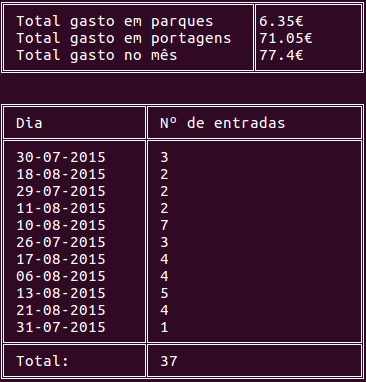
\includegraphics[scale=0.4]{terminalV1}
\break
\break
\break
\break
	De seguida, decidimos que seria possível o utilizador obter mais informações, caso desejasse.\\

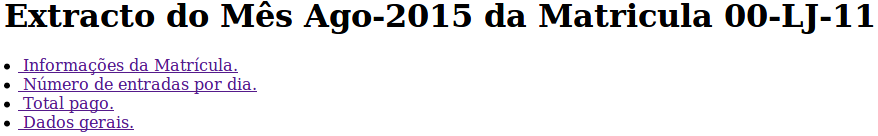
\includegraphics[scale=0.4]{htmlV2}
\break
\break
\break
\break

 	Após possibilitar a pesquisa de mais informações, decidiu-se tornar o ambiente gráfico na apresentação de resultados mais agradável. Introduzimos também a possibilidade do utilizador visualizar o percurso a que nos referíamos.\\
 
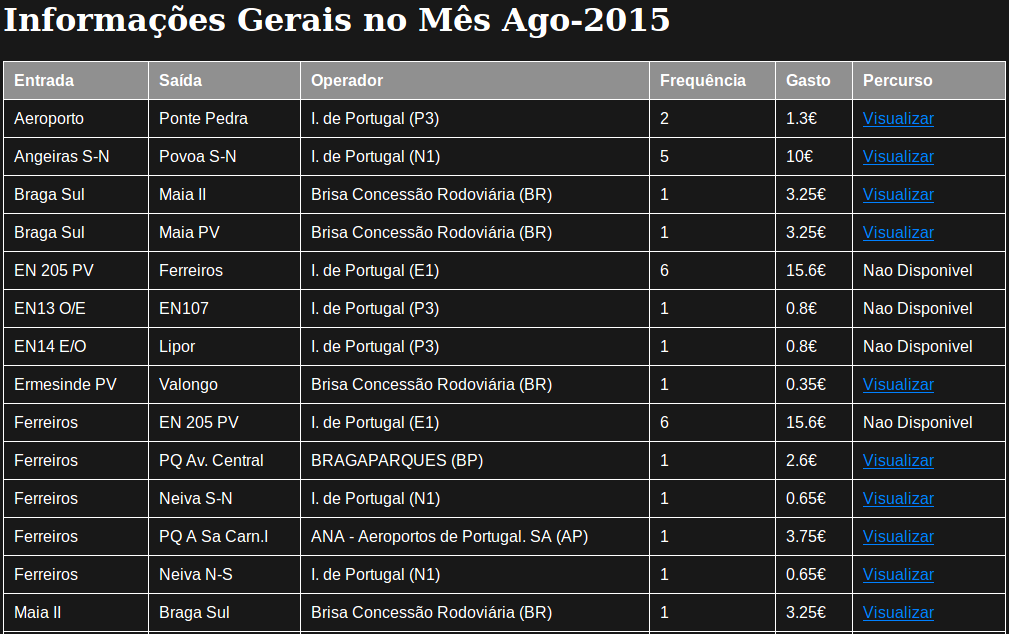
\includegraphics[scale=0.4]{htmlV3}
\break
\break
\break
\break

	Finalmente, decidimos tornar o website mais apelativo, tornando o ambiente mais navegável.\\

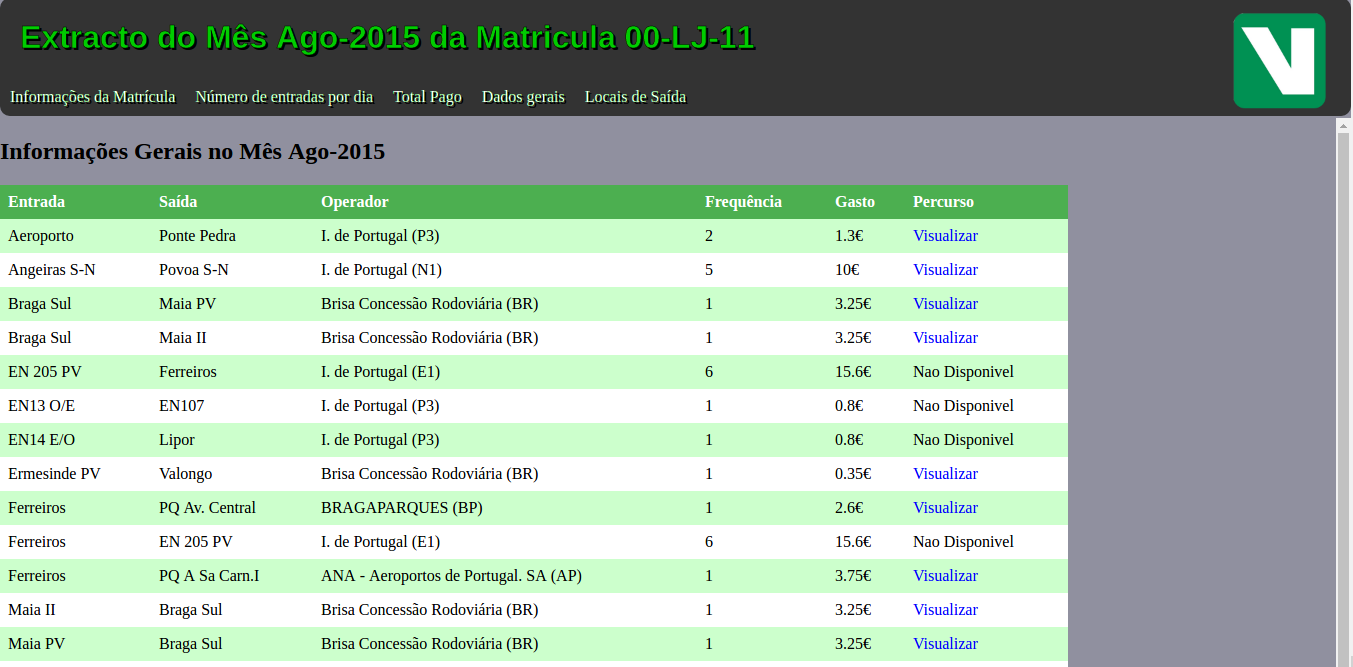
\includegraphics[scale=0.4]{html5}







\chapter{Conclusão}
	Este trabalho integra os conhecimentos adquiridos na disciplina de Processamento de Linguagens, relacionados com o uso de expressões regulares e comando \textit{gawk}.\\
\break
	Conseguimos desenvolver um \textit{script} que fosse simples e capaz de fornecer ao utilizador, todo tipo de informação disponível no ficheiro \textit{xml}. Enaltecemos o nosso agrado relativamente à forma como apresentamos os dados ao utilizador.\\
\break
	Futuramente seria abordada a possibilidade de povoamento do ficheiro \textit{xml}, integrando mais clientes e mais informação no geral.\\





\end{document}
